\documentclass{article}

\usepackage{graphicx}
\usepackage{enumitem}
\usepackage{color}
\usepackage{verbatim}
\usepackage{environ}
\usepackage{mathtools}

\usepackage{fvrb-ex}

\usepackage{eurosym}
\usepackage{amstext} % for \text
\DeclareRobustCommand{\officialeuro}{%
  \ifmmode\expandafter\text\fi
  {\fontencoding{U}\fontfamily{eurosym}\selectfont e}}


\fvset{gobble=0,numbersep=3pt}
\fvset{numbers=left,frame=single}
%\RecustomVerbatimEnvironment{Verbatim}{Verbatim}{commandchars=§µ¶}
\DefineVerbatimEnvironment%
{CVerbatim}{Verbatim}
{fontfamily=tt,fontsize=\small,frame=single,formatcom=\color{blue},label=\emph{Stata code/output}}
\DefineVerbatimEnvironment{Sinput}{Verbatim}{fontshape=sl,formatcom=\color{blue}}

\begin{document}

\title{\small Applied Panel Econometrics (MPP-E1161) - Winter Term 2015 \\ Prof. Dr. Kerstin Bernoth \\ \bigskip \Large Take Home Exam 1}
\author{Max Callaghan}
\date{October 2015}
\maketitle

\section{Part I: Basic Questions [14pt: each 2pt]}
Briefly explain why your chosen answer is correct.
\begin{enumerate}
  \item
  \begin{description}
    \item[Question] \hfill \\
    False or true: To judge, whether adding an additional explanatory variable improves the model, I check, whether the $R^{2}$ increases.
    \item[Answer] \hfill \\
    This is true to an extent. The $R^2$ describes how much of the variation in the dependent variable is explained by variation in the independent variables. Therefore, when the $R^2$ increases, our model is explaining more of the variation in the independent variable. Nevertheless, one should avoid `$R^2$ Maximising', especially if explanatory variables are added to the model without theoretical justification. Adding explanatory variables will \textit{always} increase the $R^2$, even if this is just due to chance. The Adjusted $R^2$ adjusts $R^2$ according to the number of predictors, and can help in avoiding overfitting the model
  \end{description}
  
  \item
  \begin{description}
    \item[Question] \hfill \\
    False or true: When the panel-specific factors $a_i$ are significant, the fixed-effects estimator will be preferred over pooled OLS.
    \item[Answer] \hfill \\
    True. In a fixed effects model, time-invariant factors are captured by $a_i$. Where these are significant we can say that the fixed effects captured by $a_i$ are unobservable time-invariant differences across individuals. If these are present, then it is likely that the assumption of i.i.d of our error terms is very likely violated in a pooled OLS model. It is also likely, if the unobservable characteristics of each individual panel observation are correlated with the observable characteristics in our model, that the assumption of exogeneity of the regressors is also very likely violated.
  \end{description}
  
  \item
  \begin{description}
    \item[Question] \hfill \\
    False or true: I cannot reject a Null-hypothesis on a single coefficient, when the absolute value of the $t$-statistic is smaller than the critical value.
    \item[Answer] \hfill \\
    True. At a given sample size and probability threshold, the critical value states the minimum value of $t$ at which we can reject a Null-hypothesis. If $t$ is above the critical value, we can reject the Null-hypothesis that the coefficient is not statistically significant, and if it is lower, we cannot reject it.
  \end{description}
  
  \item
  \begin{description}
    \item[Question] \hfill \\
    False or true: The OLS estimators $\beta_h$ become more accurate, when the variance of the independent variable $x_{hit}$ decreases
    \item[Answer] \hfill \\
    The accuracy of the esitamated coefficient is determined by 
    
    \begin{displaymath}
    \hat{Var}(\hat{\beta}_{h}) = \frac{\hat{\sigma}_{\epsilon}^{2} \frac{1}{NT}} {(1 - R)^{2}_{h}Var(x_{it}) }
    \text{ for } k = 1,\ldots,k
    \end{displaymath}
    
    Therefore, when the variance of $x$ decreases, the estimators $\beta_h$ become less accurate.
    
  \end{description}
  
  \item
  \begin{description}
    \item[Question] \hfill \\
    Calculate the $R^2$ of a regression, of which the variance of the realized variable $y$ is equal to 6.4 and the variance of the fitted dependent variable $\hat{y}$ is 5.8
    \item[Answer] \hfill \\
    The $R^2$ is given by
    \[R^2 = \frac{Var(\hat{y})}{Var(y)} = 0.91 \] 
  \end{description}
  
  \item
  \begin{description}
    \item[Question] \hfill \\
    False or true: Including an irrelevant variable does not lead to biased OLS coefficients.
    \item[Answer] \hfill \\
    Including irrelevant variables does not lead to biased OLS coefficients in the relevant variables. It can only make the model less efficient. If the true model is $y$
  \end{description}
  
  \item
  \begin{description}
    \item[Question] \hfill \\
    False or true: When a regressor is endogenous, we have the situation that the dependent variable $y_{it}$ is correlated with the residual $\epsilon_{it},cov(y_{it},\epsilon_{it}) \neq 0$.
    \item[Answer] \hfill \\
    True. That is the definition of an endogeneity problem, in can either be a simultaneity problem, or an omitted variable problem.
  \end{description}
  
\end{enumerate}

\section{Part 2: GDP Growth and Investment [28pt]}

\begin{enumerate}
  \item
  \begin{description}
    \item[Question] \hfill \\
    Calculate the variances of the GDP growth ($Var(y_{it})$) and investment ($Var(x_{it})$) and their covariance ($Cov(x_{it},y_{it})$).
    \item[Answer] \hfill \\
    \begin{itemize}
      \item Population variance of GDP Growth: $\frac{1}{NT} \sum^{N}_{i=1} \sum^{N}_{t=1} (y_{it}-\bar{y}^{2}) = 63.75$
      \item Population variance of Investment: $\frac{1}{NT} \sum^{N}_{i=1} \sum^{N}_{t=1} (x_{it}-\bar{x}^{2}) = 9.93$
    \end{itemize}
  \end{description}
  
  \item
  \begin{description}
    \item[Question] \hfill \\
    Calculate the OLS solution for $\hat{\beta}_{0}$ and $\hat{\beta}_{1}$ and write-up the regression equation.
    \item[Answer] \hfill \\
    $\hat{\beta}_{1} = \frac{Cov(x_{it},y_{it})}{Var(x_{it})}$ and $\hat{\beta}_{0} = \bar{y} - \hat{\beta}_{1}\bar{x}$
    
    $\hat{\beta}_{1} = 0.335744$ and $\hat{\beta}_{0} = -3.9314909$
    
    $GDPgrowth_{it} = -3.93 + 0.34Investment_{it}$
  \end{description}
  
  \item
  \begin{description}
    \item[Question] \hfill \\
    Give an interpretation of the estimated coefficients $\hat{\beta}_{0}$ and $\hat{\beta}_{1}$.
    \item[Answer] \hfill \\
    The estimated coefficients tell us that the model predicts that when $x$ (Investment) is 0, $y$ (GDP growth) will be $\hat{\beta}_{0} = -3.93$. For every increase in $x$, $y$ is predicted to increase by $0.34$. The model estimates a positive effect of Investment on GDP growth.
  \end{description}
  
  \item
  \begin{description}
    \item[Question] \hfill \\
    Add the fitted values of $y_{it}, \hat{y}_{it} = \hat{\beta}_{0} + \hat{\beta}_{1}x_{it}$, to the table above.
    \item[Answer] \hfill \\
    See excel sheet.
  \end{description}
  
  \item
  \begin{description}
    \item[Question] \hfill \\
    Calculate the residuals and add them into the table above.
    \item[Answer] \hfill \\
    See excel sheet. $\epsilon_{it} = \hat{y}_{it} - y_{it}$
  \end{description}
  
  \item
  \begin{description}
    \item[Question] \hfill \\
    Draw the regression line into the graph below and mark explicitly, where the regression line cross the $y$ axis and the slope.
    \item[Answer] \hfill \\
    The graph given in the exam is substituted for a similar graph produced by excel that extends the y axis so that the intercept can be drawn.
    \begin{figure}
      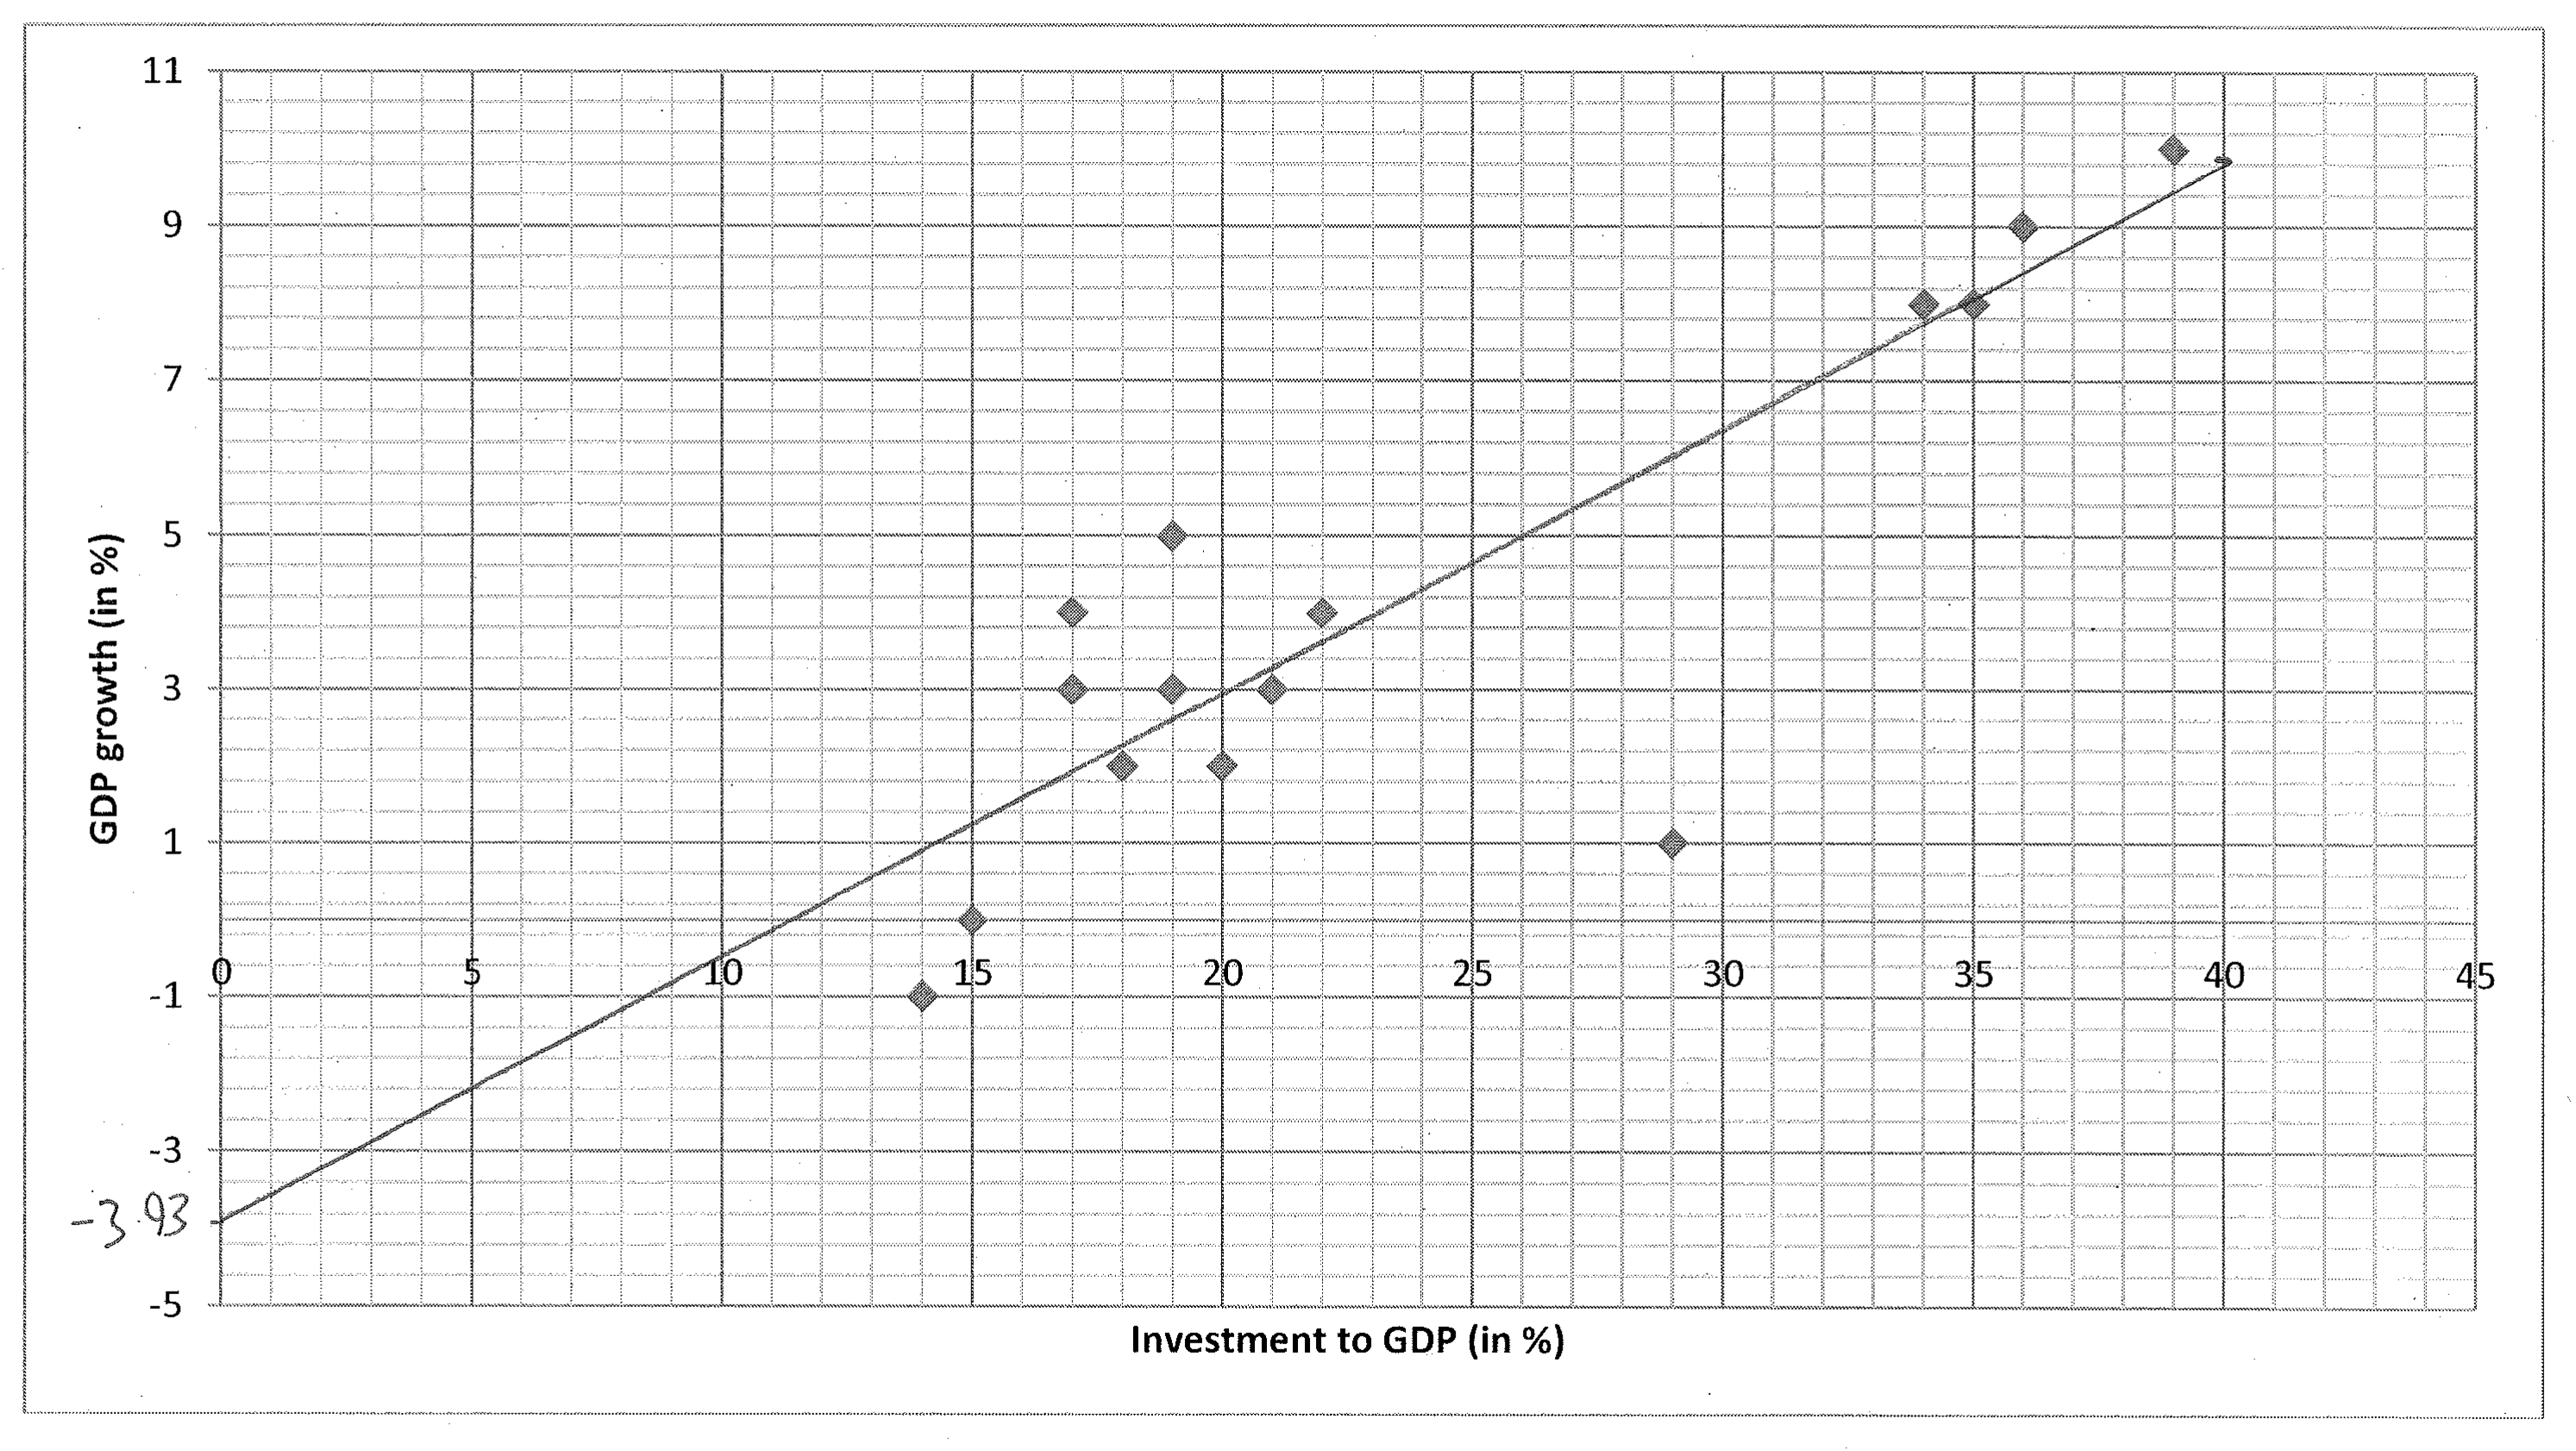
\includegraphics[width=12cm]{../graph_scan-1.png}
      \caption{Intercept = -3.93, Slope = 0.34}
    \end{figure}
  \end{description}
  
  \item
  \begin{description}
    \item[Question] \hfill \\
    Use graphical inspection to judge, whether this regression suffers from heteroscedasticity.
    \item[Answer] \hfill \\
    It is difficult to make a judgement with so few data points, but the variance at high values of x seems to be smaller than the variance at low values of x. This suggests that the data is, at least to some extent, heteroscedastic.
  \end{description}
  
  \item
  \begin{description}
    \item[Question] \hfill \\
    Calculate the standard errors of $\hat{\beta}_{1}$ (Note: The standard error is the square root of their variances: $s.e.\hat{\beta}_{1} = \sqrt{\hat{Var}(\hat{\beta}_{1})}$).
    \item[Answer] \hfill \\
    $$ s.e.\beta_{1}= \sqrt{\frac{\frac{1}{n-2}\sum_{i=1}^{N}\sum_{t=1}^{T}{\hat{\epsilon}^2_{it}}}{\sum_{i=1}^{N}\sum_{t=1}^{T}(x_{it}-\bar{x})^2}} = 0.055$$
  \end{description}
  
  \item
  \begin{description}
    \item[Question] \hfill \\
    Perform a $t$-test at the 5\% significance level to test the hypothesis that the level of investment has a positive impact on GDP growth. Thus, the Null Hypothesis is $H_{0} : \beta_{1} = 0$. Interpret the result.
    \item[Answer] \hfill \\
    The $t$-statistic of our hypothesis is given by
    $$ t = \frac{\hat{\beta}_1-\hat{\beta}^0_1}{s.e.\hat{\beta}_1} = \frac{0.34-0}{0.055} = 6.18$$
    Our degrees of freedom are $df = NT - k = 16-1 = 15$
    
    With 15 degrees of freedom, the citical value for a $t$-test at the 5\% significance level  is $2.131$.
    
    Since 6.18 is larger than 2.131, we can reject the null hypothesis that the level of investment has no impact on GDP growth.
  \end{description}
  
  \item
  \begin{description}
    \item[Question] \hfill \\
    Calculate the $R^2$ of the regression and interpret the result (Hint: Choose the formula, which seems most convenient given the variables you already have at hand).
    \item[Answer] \hfill \\
    $R^2 = 1 - \frac{Var(\hat{\epsilon})}{Var(y)} = 0.72$
  \end{description}
  
\end{enumerate}

\section{Part 3: Current Account Imbalances and Exchange Rate Regimes [37pt]}

\subsection{Regression preparation [6pt]}
  \begin{enumerate}[label=(\alph*)]
    \item 
    \begin{description}
      \item[Question] \hfill \\
      Explain briefly, why we should concentrate on the \textit{absolute} value and not the level of the current account to measure current account imbalances.
      \item[Answer] \hfill \\
      We want to look at current account imbalances. Variation either side of 0 is an imbalance, so we look at the absolute value, and take that as the size of the current account imbalance, regardless of direction.
    \end{description}
    \item
    \begin{enumerate}[label=(\roman*)]
      \item 
      \begin{description}
        \item[Question] \hfill \\
        \textit{abs\_cagdp}: A variable that depicts the absolute value of $cagdp$ $ (|cagdp|$) (Hint: Use Stata help to find out the command to calculate absolute values).
        \item[Answer] \hfill \\
        \begin{CVerbatim}
  cap gen abs_cagdp = abs(cagdp)
        \end{CVerbatim}
      \end{description}
      \item 
      \begin{description}
        \item[Question] \hfill \\
        \textit{trade\_openness}: A variable that measures nominal export relative to GDP plus nominal import to GDP $(imports+exports)$.
        \item[Answer] \hfill \\
        \begin{CVerbatim}
  cap gen trade_openness = importsgdp + exportsgdp
        \end{CVerbatim}
      \end{description}
    \end{enumerate}
    \item 
    \begin{description}
      \item[Question] \hfill \\
      We want to focus only on industrial countries. Thus, drop all non-industrial countries from the data set. Indicate, how many observations you have left in your data set.
      \item[Answer] \hfill \\
      \begin{CVerbatim}
  drop if ind == 0
  (1,465 observations deleted)
      \end{CVerbatim}
    \end{description}
  \end{enumerate}
  
\subsection{Model Choice [8pt]}
To test your hypothesis, you want to run a pooled OLS regresssion with \textit{abs\_gdp} as dependent variable and regime, \textit{exportsgdp, trade\_openess, finance, gdpgrowth} as independent variables
  \begin{enumerate}[label=(\alph*)]
    \item 
    \begin{description}
      \item[Question] \hfill \\
      Explain, why we do not regress simply the \textit{abs\_cagdp} on \textit{regime}, but also add other control variables to the set of regressors? What could be the consequences for the estimators, if one ignores important explanatory variables
      \item[Answer] \hfill \\
      If regime type was the only variable that we thought had an effect on \textit{abs\_cagdp}, we would only include regime type. If other variables affect our dependent variable and we do not include them, we risk \textit{omitted variable bias}. When we miss out an independent variable that is both a determinant of the dependent variable \textit{and} correlated with one or more of our independent variables, the coefficient for the included independent variable will be biased because it will contain part of the effects of omitted variables that are correlated with our included variable.
    \end{description}
  \end{enumerate}
  
  \begin{enumerate}[label=(\alph*)]
    \item 
    \begin{description}
      \item[Question] \hfill \\
      Explain, what the consequences are, if we have a multicollinearity problem among the explanatory variables
      \item[Answer] \hfill \\
      Multicollinearity describes a model where the independent variables are correlated with each other. In a case of perfect multicollinearity, there is a linear relationship between at least two of the variables.
      
      The variance of the estimated coefficients is given by
      
      \begin{displaymath} 
      \hat{Var}(\hat{\beta}_h) = \frac{\hat{\sigma}^2_{\epsilon}\frac{1}{NT}}{(1-R^2_h)Var(x_{it})} \text{ for } k=1,\ldots,k
      \end{displaymath}
      
      The greater the relationship between \(x_{it}\) and the other independent variables (given by \(R^2_h\)), the greater the variance of our estimator. Multicollinearity makes our estimators less precise.
    \end{description}
  \end{enumerate}
  
  \begin{enumerate}[label=(\alph*)]
    \item 
    \begin{description}
      \item[Question] \hfill \\
      Test, whether we have a multicollinearity problem between our explanatory variables. Explain, how you derive your conclusion.
      \item[Answer] \hfill \\
      Stata calculates the Variance Inflation Factor (VIF) for us using the formula
      
      \[ VIF(\hat{\beta}_h) = \frac{1}{1-R^2_h} \]
      
      High values for VIF indicate the presence of multicollinearity. 10 is sometimes used as a cutoff point.
      
      \begin{CVerbatim}
. estat vif

    Variable |       VIF       1/VIF  
-------------+----------------------
trade_open~s |    118.93    0.008408
  exportsgdp |    116.98    0.008548
     finance |      1.40    0.712628
      regime |      1.20    0.834933
   gdpgrowth |      1.13    0.886961
-------------+----------------------
    Mean VIF |     47.93
      \end{CVerbatim}
      Unsurprisingly, we can detect multicollinearity problems in the high VIF values for both trade openness and exportsgdp. This is because we created trade openness out of a linear combination of exports and imports. So, notwithstanding some degree of variation between the balance or otherwise of exports and imports, they are highly correlated
    \end{description}
  \end{enumerate}
  
  \begin{enumerate}[label=(\alph*)]
    \item 
    \begin{description}
      \item[Question] \hfill \\
      In case you do detect multicollinear variables: What would you recomment to do? Which of the potential multicollinear variables would you drop?
      \item[Answer] \hfill \\
      We created the variable \textit{tradeopenness}, presumably, because we thought that the combination of both exports and imports had an effect on our dependent variable. If we drop it, we are left with just imports; if we drop imports, than we still have the effect of the combination of exports and imports. An alternative would be to use imports and exports separately, but they would most likely still be highly correlated, though to a lesser extent.
    \end{description}
  \end{enumerate}
  
\subsection{Estimating a pooled OLS regression [15pt]}
  
  \begin{enumerate}[label=(\alph*)]
    \item 
    \begin{description}
      \item[Question] \hfill \\
      Continue with your preferred set of regressors (meaning: drop if necessary a variable(s) to solve for a potential multicollinearity problem (see Question 2.c)) and estimate the determinants of \textit{abs\_cagdp} with \textit{pooled OLS}.
      \item[Answer] \hfill \\
      \begin{CVerbatim}
reg abs_cagdp regime trade_openness finance gdpgrowth
outtex, file(pooled.tex) labels level detail ///
  legend key(stab) replace
      \end{CVerbatim}
      
{
\def\onepc{$^{\ast\ast}$} \def\fivepc{$^{\ast}$}
\def\tenpc{$^{\dag}$}
\def\legend{\multicolumn{4}{l}{\footnotesize{Significance levels
:\hspace{1em} $\dag$ : 10\% \hspace{1em}
$\ast$ : 5\% \hspace{1em} $\ast\ast$ : 1\% \normalsize}}}
\begin{table}[htbp]\centering
 \caption{Estimation results : regress
\label{stab}}
\begin{tabular}{l r @{} l c }\hline\hline 
\multicolumn{1}{c}
{\textbf{Variable}}
 & \multicolumn{2}{c}{\textbf{Coefficient}}  & \textbf{(Std. Err.)} \\ \hline
0b.regime  &  0.000&  & (0.000)\\
1.regime  &  -1.342&\onepc  & (0.305)\\
2.regime  &  -1.363&\onepc  & (0.316)\\
trade\_openness  &  0.029&\onepc  & (0.002)\\
finance  &  0.025&  & (0.091)\\
gdpgrowth  &  0.101&\fivepc  & (0.049)\\
Intercept  &  2.236&\onepc  & (0.318)\\
\hline\multicolumn{4}{c}{}\\
\hline N & \multicolumn{3}{c}{818}\\
R$^{2}$ & \multicolumn{3}{c}{0.218}\\
F $ _{(5,812)}$ & \multicolumn{3}{c}{45.368}\\
\hline\legend
\end{tabular}
\end{table}
}


    \end{description}
  \end{enumerate}
  
  \begin{enumerate}[label=(\alph*)]
    \item 
    \begin{description}
      \item[Question] \hfill \\
      Indicate, whether the `Friedman hypothesis' is supported by the data or not.
      \item[Answer] \hfill \\
      The `Friedman hypothesis' suggested that ``fixed exchange rate ragimes should facilitate the build-up of current account imbalances''
      We create dummy variables of the `intermediate' and `fixed regime' types, compared to the reference category of `floating'. Increases in our dependent variable \textit{abs\_cagdp} indicate that the current account imbalance is larger. Therefore, if Friedman's hypothesis were correct, the coefficient of the  dummy variable for a fixed regime would be positive. 
      The data show a statistically significant negative effect of a fixed regime type compared to a floating regime type on current account imbalance. The data therefore suggest that we reject Friedman's hypothesis.
    \end{description}
  \end{enumerate}
  
  \begin{enumerate}[label=(\alph*)]
    \item 
    \begin{description}
      \item[Question] \hfill \\
      Indicate, which of the other control variables have a significant impact on current account imbalances (assume a significance level of 5\%).
      \item[Answer] \hfill \\
      Trade openness and GDP growth both have statistically significant positive effects on current account imbalances.
    \end{description}
  \end{enumerate}
  
  \begin{enumerate}[label=(\alph*)]
    \item 
    \begin{description}
      \item[Question] \hfill \\
      Give a numerical interpretation of the estimated coefficients.
      \item[Answer] \hfill \\
      The constant is 1.841728, so if all variables were equal to 0, the model would predict an absolute current account as a percentage of GDP (\textit{abs\_cagdp}) value of 1.84. 
      
      Compared to the reference category `floating', observations that are in the category `intermediate' are predicted to have a \textit{abs\_cagdp} that is lower by 1.34. Observations that are in the category `fixed' are predicted to have a \textit{abs\_cagdp} that is lower by 1.36.
      
      A one unit increase in \textit{finance} is predicts a 0.02 increase in \textit{abs\_cagdp}
      
      A one unit increase in GDP growth predicts a .1 unit increase in \textit{abs\_cagdp}.

    \end{description}
  \end{enumerate}
  
  \begin{enumerate}[label=(\alph*)]
    \item 
    \begin{description}
      \item[Question] \hfill \\
      Explain whther the signs of the estimated coefficients make sense from an economic point of view.
      \item[Answer] \hfill \\
      One might expect, following Milton and Miltonians, the opposite. Openness to trade and to capital flow are usually cited as \textit{good things} for countries' economies. Openness in general should, according to Milton, lead to reduced capital imbalances. The data don't bear this out. GDP Growth may make more economic sense, as, following the `Friedman hypothesis', more growth may lead to more consumption, leading to more imports.
    \end{description}
  \end{enumerate}

\subsection{Estimating a fixed-effects regression [8pt]}

  \begin{enumerate}[label=(\alph*)]
    \item 
    \begin{description}
      \item[Question] \hfill \\
      Perform a Breusch-Pagan LM test for heteroscedasticity and interpret the result.
      \item[Answer] \hfill \\
      \begin{CVerbatim}
. estat hettest

Breusch-Pagan / Cook-Weisberg test for heteroskedasticity 
         Ho: Constant variance
         Variables: fitted values of abs_cagdp

         chi2(1)      =    48.68
         Prob > chi2  =   0.0000
      \end{CVerbatim}
    \end{description}
  \end{enumerate}
  
  \begin{enumerate}[label=(\alph*)]
    \item 
    \begin{description}
      \item[Question] \hfill \\
      Estimate your regression model this time with a \textit{fixed-effects panel} estimation.
      \item[Answer] \hfill \\
      \begin{CVerbatim}
xtreg abs_cagdp regime trade_openness finance gdpgrowth, fe
outtex, file(fe.tex) labels level detail ///
	legend key(stab) replace
      \end{CVerbatim}
      
{
\def\onepc{$^{\ast\ast}$} \def\fivepc{$^{\ast}$}
\def\tenpc{$^{\dag}$}
\def\legend{\multicolumn{4}{l}{\footnotesize{Significance levels
:\hspace{1em} $\dag$ : 10\% \hspace{1em}
$\ast$ : 5\% \hspace{1em} $\ast\ast$ : 1\% \normalsize}}}
\begin{table}[htbp]\centering
 \caption{Estimation results : xtreg
\label{stab}}
\begin{tabular}{l r @{} l c }\hline\hline 
\multicolumn{1}{c}
{\textbf{Variable}}
 & \multicolumn{2}{c}{\textbf{Coefficient}}  & \textbf{(Std. Err.)} \\ \hline
regime  &  -0.139&  & (0.213)\\
trade\_openness  &  0.038&\onepc  & (0.008)\\
finance  &  0.391&\onepc  & (0.100)\\
gdpgrowth  &  0.068&  & (0.046)\\
Intercept  &  0.411&  & (0.614)\\
\hline\multicolumn{4}{c}{}\\
\hline N & \multicolumn{3}{c}{818}\\
R$^{2}$ & \multicolumn{3}{c}{0.074}\\
F $ _{(32,785)}$ & \multicolumn{3}{c}{15.658}\\
\hline\legend
\end{tabular}
\end{table}
}


    \end{description}
  \end{enumerate}
  
  \begin{enumerate}[label=(\alph*)]
    \item 
    \begin{description}
      \item[Question] \hfill \\
      Indicate again, whether the `Friedman hypothesis' is supported this time by the data or not.
      \item[Answer] \hfill \\
      In this case, the sign is still negative, contradicting the `Friedman hypothesis'. However, the coefficient for the dummy variable `fixed' is not statistically significant, so we cannot reject Friedman's hypothesis that there is a positive relationship. 
    \end{description}
  \end{enumerate}
  
  \begin{enumerate}[label=(\alph*)]
    \item 
    \begin{description}
      \item[Question] \hfill \\
      What could explain the different results you find for the variable \textit{regime} once you estimate a fixed-effects regression instead of pooled OLS?
      \item[Answer] \hfill \\
      The coefficient was smaller with a fixed effects model, which suggests that there could be a variable which is positively correlated with regime type and negatively correlated with current account imbalances. The standard error is also larger, which could suggest that there was less variance in regime type (x) when we look at effects within countries. 
    \end{description}
  \end{enumerate}

\section{Model Interpretation [6pt]}
  
  \begin{enumerate}
    \item 
    \begin{description}
      \item[Question] \hfill \\
      \[Wage_{\euro/hour} = 8.71 + 1.50 Education_{Years} - 0.1 Education^2_{Years} + \epsilon\]
      \item[Answer] \hfill \\
      The intercept tells us that when education is 0 years, the model predicts that the wage in euros per hour will be 8.71.
      
      The first beta coefficient tells us that for each increase in years of education, wage in euros will increase by 1.50 euros per hour.
      
      The second beta coefficient tells us that for each increase in the squared value of education, wages will decrease by 0.1 euros per hour.
    \end{description}
  
    \item 
    \begin{description}
      \item[Question] \hfill \\
      \[ln(Wage_{\euro/hour}) = 2.10 + 0.11 Education_{Years} + \epsilon\]
      \item[Answer] \hfill \\
      The intercept tells us that when education is 0, the log of wages in euros per hour will be 2.10. If we take the exponential of 2.10, we see that the actual value will be 8.17.
      
      The first beta coefficient tells us that for each unit increase in years of education, wages in euros per hour will increase by 11\%.
    \end{description}
    
    \item 
    \begin{description}
      \item[Question] \hfill \\
      \[Inflation_{in \%} = 8.71 + 1.50 GDPGrowth_{in \%} + \epsilon \] 
      \item[Answer] \hfill \\
      The intercept tells us that when GDP Growth is 0\%, Inflation will be 8.71 \%.
      
      The beta coefficient tells us that for each percentage point increase in GDP growth in \%, Inflation will increase by 1.5 percentage points.
    \end{description}
  \end{enumerate}





\end{document}